% Created 2021-12-04 sam. 16:08
% Intended LaTeX compiler: pdflatex
\documentclass[10pt]{beamer}
\usepackage[utf8]{inputenc}
\usepackage[T1]{fontenc}
\usepackage{graphicx}
\usepackage{grffile}
\usepackage{longtable}
\usepackage{wrapfig}
\usepackage{rotating}
\usepackage[normalem]{ulem}
\usepackage{amsmath}
\usepackage{textcomp}
\usepackage{amssymb}
\usepackage{capt-of}
\usepackage{hyperref}
\usepackage{minted}
\setlength{\parskip}{5pt}
\newcommand{\footnoteframe}[1]{\footnote[frame]{#1}}
\addtobeamertemplate{footnote}{}{\vspace{2ex}}
\usepackage{tabularx}
\usetheme{Berkeley}
\author{Jay Morgan}
\date{11th October 2021}
\title{Programming Level-up}
\subtitle{An Introduction to using Linux}
\hypersetup{
 pdfauthor={Jay Morgan},
 pdftitle={Programming Level-up},
 pdfkeywords={},
 pdfsubject={},
 pdfcreator={Emacs 27.1 (Org mode 9.4.6)}, 
 pdflang={English}}
\begin{document}

\maketitle
\begin{frame}{Outline}
\tableofcontents
\end{frame}


\section{Linux}
\label{sec:org2adc12d}

\subsection{What is Linux}
\label{sec:org84823dc}

\begin{frame}[label={sec:org0100c76}]{What is Linux?}
\begin{itemize}
\item Linux is a popular operating system (OS) like Windows, or MacOS.
\item Unlike these other two OSs, Linux is open source, which means the source code
is freely available to look at and modify.
\item As its open source, its very possible for anyone to build their \emph{own} version of
Linux or build on top of Linux to create their own \emph{Distribution} of Linux.
\end{itemize}
\end{frame}

\begin{frame}[label={sec:orgfbd376d}]{What's a Distribution?}
A distribution can be considered like a \emph{flavour} or version of Linux. There are
many popular flavours that attempt to meet different needs from different
users. For example:

\begin{itemize}
\item Ubuntu -- typically the first Linux experience people will have. Attempts to be
very user friendly.
\item Fedora -- stable and secure distribution while also providing up-to-date packages.
\item Arch Linux -- strong focus on customisability rather than user friendliness
with bleeding edge packages.
\end{itemize}
\end{frame}

\begin{frame}[label={sec:orgfddf0a6}]{What's a Distribution?}
\begin{center}
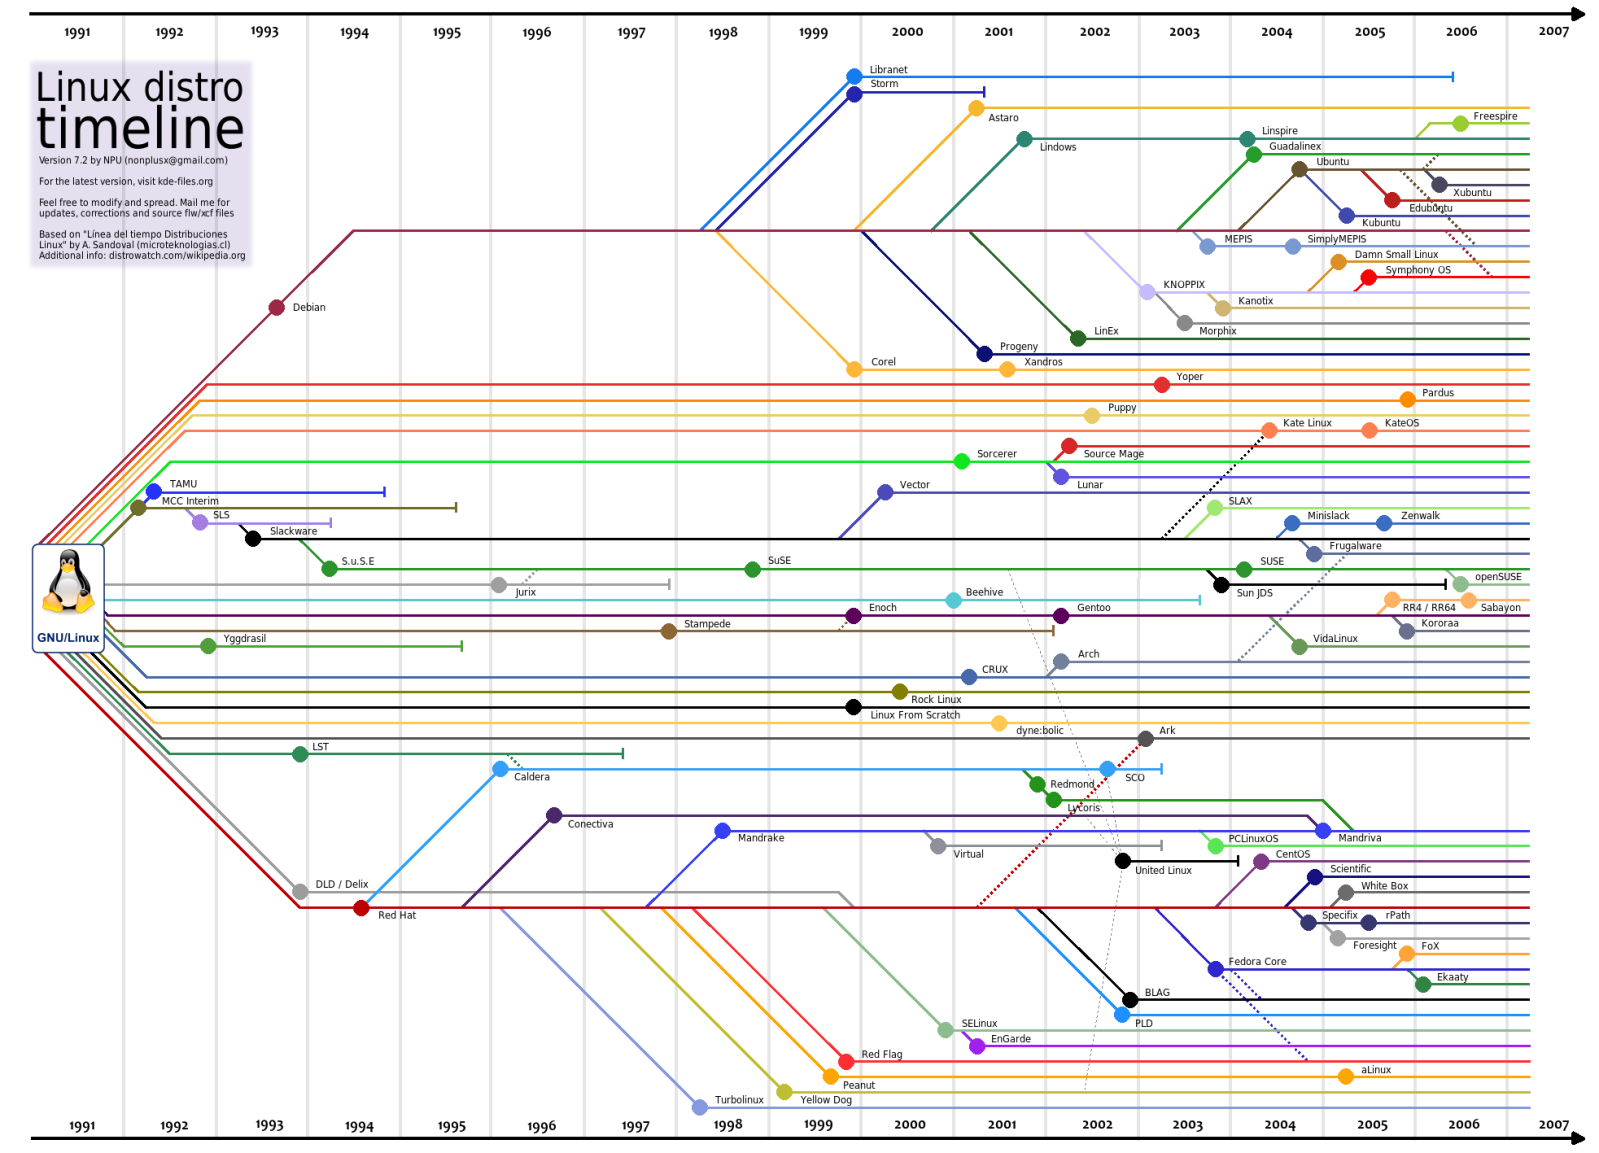
\includegraphics[width=\textwidth]{images/family-tree.png}
\end{center}
\end{frame}

\begin{frame}[label={sec:org31125f0}]{Defining Traits of Linux}
While we have said that Linux is open source, there are many other traits that
make it stand out from other operating systems:

\begin{itemize}
\item Complete control of how the system operates.
\item The level of flexibility and automation that you can get from using the Linux
command line.
\end{itemize}

While there are many other traits, these two are going to be what we're going to
focus on.
\end{frame}

\subsection{The command line}
\label{sec:org2fab867}

\begin{frame}[label={sec:orge64410f},fragile]{What's a command?}
 While many recent versions of Linux makes things more accessible via GUIs, they
will never be a substitute for using the command line. We're going to learn how
to control the system via the command line, via a \alert{shell}. A shell, like the
Python REPL we've already seen, is waits for you to input commands, executes the
command, and prints the output if there is output to print.

A Linux command is a call to a program optionally followed by some
arguments. For example, if we want list out the files and folders in the
directory, we would use the \texttt{ls} (list) command:

\begin{minted}[frame=lines,linenos=true,firstnumber=last,fontsize=\footnotesize,xleftmargin=15pt,numbersep=8pt]{bash}
ls
\end{minted}
\end{frame}

\begin{frame}[label={sec:orge74d96d},fragile]{What is a command?}
 The \texttt{ls} command comes with a number of optional flags and arguments that we can
add onto the call. When calling a command a flag is something that begins with a
\texttt{-} , for example \texttt{-l} tells \texttt{ls} to list the directory in a list format.

\begin{minted}[frame=lines,linenos=true,firstnumber=last,fontsize=\footnotesize,xleftmargin=15pt,numbersep=8pt]{bash}
ls -l
\end{minted}
\end{frame}

\begin{frame}[label={sec:orga5ea721},fragile]{What is a command?}
 We have supplied the \texttt{-l} flag. There are many other flags for \texttt{ls}, like for
example, the human readable file systems with \texttt{-h} or show hidden files (files
that start with a period) with \texttt{-a}.

When we're using multiple flags we could write

\begin{minted}[frame=lines,linenos=true,firstnumber=last,fontsize=\footnotesize,xleftmargin=15pt,numbersep=8pt]{bash}
ls -l -h -a
\end{minted}

Or:

\begin{minted}[frame=lines,linenos=true,firstnumber=last,fontsize=\footnotesize,xleftmargin=15pt,numbersep=8pt]{bash}
ls -lha
\end{minted}
\end{frame}

\begin{frame}[label={sec:org4b5ad96},fragile]{What is a command?}
 Sometimes commands take optional positional arguments. Going back to our list
directory command, where, by default, it will list the current directory. But
instead we can tell the command to list a particular directory by supplying the
path as an argument

\begin{minted}[frame=lines,linenos=true,firstnumber=last,fontsize=\footnotesize,xleftmargin=15pt,numbersep=8pt]{bash}
ls images/ -lha
# or ls -lha images/ works too
\end{minted}
\end{frame}

\begin{frame}[label={sec:org9be221c},fragile]{What is a command?}
 How do I know how to use a command? Well that's where another command comes
in. It's called \texttt{man} (short for manual). If you pass another command to the \texttt{man}
command, the documentation will be shown in the terminal, e.g.:

\begin{minted}[frame=lines,linenos=true,firstnumber=last,fontsize=\footnotesize,xleftmargin=15pt,numbersep=8pt]{bash}
man ls  # display the documentation for ls
\end{minted}

The documentation should list all the different flags and arguments, describe
what they mean, and sometimes give example or most common usage of a command.

When the 'man page' is display, you can scroll up and down the page using your
arrow keys, and page-up and page-down. When you're done reading, just hit the
'q' character
\end{frame}

\begin{frame}[label={sec:orgd163f4c},fragile]{Very useful commands}
 I am going to go through some of the most common commands just to make sure that
you're familiar with the typical usage.

We've already seen \texttt{ls} to list a directory. The command to move to a directory is
\texttt{cd} (change directory), that takes an argument of filepath to move to:

\begin{minted}[frame=lines,linenos=true,firstnumber=last,fontsize=\footnotesize,xleftmargin=15pt,numbersep=8pt]{bash}
cd ~ # tilde is short-hand for the 'home directory'
cd ~/Documents/My\ Files  # go to Documents and then to "My Files"
cd   # no argument, by default goes to the home directory
\end{minted}
\end{frame}

\begin{frame}[label={sec:orga7930d4},fragile]{Very useful commands -- mkdir}
 Sticking with the them of directories, to make a new directory we use \texttt{mkdir},
whose argument takes the name of the directory we want to create:

\begin{minted}[frame=lines,linenos=true,firstnumber=last,fontsize=\footnotesize,xleftmargin=15pt,numbersep=8pt]{bash}
mkdir my_new_directory
\end{minted}

You can create a many level nested directory structure all at once using the \texttt{-p}
(parents) flag, that tells \texttt{mkdir} if the parent directory of the target directory
doesn't exist, create it.

\begin{minted}[frame=lines,linenos=true,firstnumber=last,fontsize=\footnotesize,xleftmargin=15pt,numbersep=8pt]{bash}
mkdir photos/2020/01/05  # won't work unless photos/2020/01 exist
mkdir -p photos/2020/01/05  # this will work
\end{minted}
\end{frame}

\begin{frame}[label={sec:org277b798},fragile]{Very useful commands -- cp}
 To copy a file or directory, we can use the \texttt{cp} command. Here we are copying a
file, where the first argument is the filepath of the file you want to copy and the second
argument is the filepath where the copy should be placed.

\begin{minted}[frame=lines,linenos=true,firstnumber=last,fontsize=\footnotesize,xleftmargin=15pt,numbersep=8pt]{bash}
cp my_old_file my_new_file
\end{minted}

By default (without a flag), \texttt{cp} will not work with directories, for that you
have to use the \texttt{-r} (recursive) flag

\begin{minted}[frame=lines,linenos=true,firstnumber=last,fontsize=\footnotesize,xleftmargin=15pt,numbersep=8pt]{bash}
cp -r data/ data-backup
\end{minted}
\end{frame}

\begin{frame}[label={sec:org50609ba},fragile]{Very useful commands -- mv}
 The syntax of moving a file is similar to that of \texttt{cp}:

\begin{minted}[frame=lines,linenos=true,firstnumber=last,fontsize=\footnotesize,xleftmargin=15pt,numbersep=8pt]{bash}
mv old_file new_file
\end{minted}

Except that it works for both files and directories without any flags. \texttt{mv} can
also be used to \alert{rename} files, that's all renaming is: moving a file to the same
directory under a different name.
\end{frame}

\begin{frame}[label={sec:org721176c},fragile]{Very useful commands -- rm}
 To remove a file us \texttt{rm}:

\begin{minted}[frame=lines,linenos=true,firstnumber=last,fontsize=\footnotesize,xleftmargin=15pt,numbersep=8pt]{bash}
rm file_to_delete
\end{minted}

If you want to delete a directory, use the \texttt{-r} (recursive) flag:

\begin{minted}[frame=lines,linenos=true,firstnumber=last,fontsize=\footnotesize,xleftmargin=15pt,numbersep=8pt]{bash}
rm -r directory_to_delete/
\end{minted}
\end{frame}

\begin{frame}[label={sec:org81e58a7},fragile]{Very useful commands -- cat}
 \texttt{cat} stands for concatenate, i.e. concatenating the contents of two or more
files:

\begin{minted}[frame=lines,linenos=true,firstnumber=last,fontsize=\footnotesize,xleftmargin=15pt,numbersep=8pt]{bash}
cat file1 file2
\end{minted}

The result is that the concatenation of these two files will be printed to the
screen. If you wanted to put the result into its own file you would redirect the
output using \texttt{>}

\begin{minted}[frame=lines,linenos=true,firstnumber=last,fontsize=\footnotesize,xleftmargin=15pt,numbersep=8pt]{bash}
cat file1 file2 > newfile
\end{minted}

Since cat reads the file and prints it to screen it is a very handy way to view
the contents of a file, even if it was not intended for that.
\end{frame}

\begin{frame}[label={sec:org1d0ae5e},fragile]{Very useful commands -- pwd}
 Sometimes you may get lost when moving directories. \texttt{pwd} prints the current
working directory from the root directory, i.e. the path that is printed is an
absolute path.

\begin{minted}[frame=lines,linenos=true,firstnumber=last,fontsize=\footnotesize,xleftmargin=15pt,numbersep=8pt]{bash}
pwd
\end{minted}
\end{frame}

\begin{frame}[label={sec:org6986597},fragile]{Very useful commands -- find}
 If we want to list all files of a certain type, we can use the wildcard \texttt{*} that
we've seen before:

\begin{minted}[frame=lines,linenos=true,firstnumber=last,fontsize=\footnotesize,xleftmargin=15pt,numbersep=8pt]{bash}
ls *.jpg # list all files that end with .jpg
\end{minted}

However, this will only list for the current directory. Perhaps the better way
to find files will be using the \texttt{find} command:

\begin{minted}[frame=lines,linenos=true,firstnumber=last,fontsize=\footnotesize,xleftmargin=15pt,numbersep=8pt]{bash}
find . -type f -name *.jpg
\end{minted}

The first argument is the directory to start the search, then we define the type
\texttt{f} being files, and then specify the name. Find will recursively search through
directories and sub-directories to find all files that match that name.
\end{frame}

\begin{frame}[label={sec:orgeead848},fragile]{Very useful commands -- grep}
 How about if we want to find files that have a certain contents? For that we can
use \texttt{grep}. Grep will read a file and print (by default) the lines that contains
your pattern. i.e.:

\begin{minted}[frame=lines,linenos=true,firstnumber=last,fontsize=\footnotesize,xleftmargin=15pt,numbersep=8pt]{bash}
grep 'Linux' lecture.org
\end{minted}

This will print the lines that contain the word Linux in lecture.org. If we just
want the matched value, we use the \texttt{-o} flag.

\begin{minted}[frame=lines,linenos=true,firstnumber=last,fontsize=\footnotesize,xleftmargin=15pt,numbersep=8pt]{bash}
grep -o '[0-9]' lecture.org
\end{minted}

This prints all occurrences of numbers in lecture.org
\end{frame}

\begin{frame}[label={sec:org7d4fc9c},fragile]{Very useful commands -- less/head/tail}
 If a file is very long, we may not want to read the file using cat, as it will
have to print the entire file. Instead we could use \texttt{less}, which will allow us to
navigate through the file, using arrow keys to move and \texttt{q} to quit.

\begin{minted}[frame=lines,linenos=true,firstnumber=last,fontsize=\footnotesize,xleftmargin=15pt,numbersep=8pt]{bash}
less filename
\end{minted}

If we just want to view the first few lines, or the last few lines of a file we
can use head/tail, respectively:

\begin{minted}[frame=lines,linenos=true,firstnumber=last,fontsize=\footnotesize,xleftmargin=15pt,numbersep=8pt]{bash}
head filename
tail -n 20 filename  # last 20 lines
tail -F filename # constantly read the file
\end{minted}
\end{frame}

\begin{frame}[label={sec:org934d655},fragile]{Very useful commands -- wc}
 Often times we just want to count the number of something. For example, if we
want to count the number of files/folders in the directory we can do:

\begin{minted}[frame=lines,linenos=true,firstnumber=last,fontsize=\footnotesize,xleftmargin=15pt,numbersep=8pt]{bash}
ls -l | wc -l
\end{minted}

We're first printing all files and folders in a list format (one per line), then
passing (\textsubscript{piping}\_) the result to \texttt{wc}, which with the \texttt{-l} line flag, is counting the
number of lines. Therefore we get a count of the number of files and
folders. Here is another example where we're counting how many times the word
bash appears in these lecture notes:

\begin{minted}[frame=lines,linenos=true,firstnumber=last,fontsize=\footnotesize,xleftmargin=15pt,numbersep=8pt]{bash}
grep -o 'bash' lecture.org | wc -l
\end{minted}
\end{frame}

\begin{frame}[label={sec:orga086ef0},fragile]{Very useful commands -- piping}
 The purpose of piping is to pass data around between commands. We have just seen
how we can pass the output of, say, the \texttt{ls} command to  the input of \texttt{wc}. This
allows use to construct very sophisticated pipelines to do some quite complex
things from the combination of very simple commands.

\begin{minted}[frame=lines,linenos=true,firstnumber=last,fontsize=\footnotesize,xleftmargin=15pt,numbersep=8pt]{bash}
find . -name '*.txt' -type f -print0 | xargs -0 grep "something"
\end{minted}
\end{frame}

\begin{frame}[label={sec:orge3664f3},fragile]{Very useful basic commands}
 In summary we have seen the following commands:

\begin{itemize}
\item \texttt{ls} - List a directory
\item \texttt{cd} - Change/move to a directory
\item \texttt{mkdir} - Make a new directory
\item \texttt{cat} - Concatenate files
\item \texttt{cp} - Copy a file/directory
\item \texttt{mv} - Move files/folders
\item \texttt{rm} - Remove files and folders
\item \texttt{pwd} - Display the current absolute path
\item \texttt{find} - Find files
\item \texttt{grep} - Find occurrences of a pattern in a file
\item \texttt{less/head/tail} - Read a file
\item \texttt{wc} - Count
\end{itemize}
\end{frame}

\section{Shell Scripting}
\label{sec:org80b5dc3}

\subsection{Writing bash scripts}
\label{sec:org3b7c139}

\begin{frame}[label={sec:org3f80e62},fragile]{Very first bash script}
 Let's start with the classic 'Hello, World' example. We'll create a new file
called 'hello.sh' and enter the following:

\begin{minted}[frame=lines,linenos=true,firstnumber=last,fontsize=\footnotesize,xleftmargin=15pt,numbersep=8pt]{bash}
#!/bin/bash

echo "Hello, World!"
\end{minted}

First thing to notice is that the first line contains what we call a 'shebang'
or 'hashbang'. It tells Linux which shell interpreter will be used to run the
script, in this case: /bin/bash

The next (non-empty) line in the file is \texttt{echo 'Hello, World'}. This is exactly
the same as the other commands we've just seen.
\end{frame}

\begin{frame}[label={sec:org5a8cb96},fragile]{Very first bash script}
 Now that we've created and saved our bash script, we will want to run it. We
have two alternative methods to run this script:

\begin{minted}[frame=lines,linenos=true,firstnumber=last,fontsize=\footnotesize,xleftmargin=15pt,numbersep=8pt]{bash}
bash hello.sh  # run the script via bash
\end{minted}

The second, requires that we have executable privileges for the script:

\begin{minted}[frame=lines,linenos=true,firstnumber=last,fontsize=\footnotesize,xleftmargin=15pt,numbersep=8pt]{bash}
chmod +x hello.sh  # add executable 'x' privileges
./hello.sh  # execute it
\end{minted}
\end{frame}

\begin{frame}[label={sec:org43aec6f},fragile]{Variables}
 The variables we create in our bash scripts are very much the same as the
environment variables we've seen before. Take for example:

\begin{minted}[frame=lines,linenos=true,firstnumber=last,fontsize=\footnotesize,xleftmargin=15pt,numbersep=8pt]{bash}
#!/bin/bash
AGE="35"
PERSON_NAME="Jane"
echo "$PERSON_NAME is $AGE years old"
\end{minted}

We create a variable \texttt{AGE} with the \texttt{=} assignment operator. \alert{Note} we don't put
spaces either side of the equals sign in bash. To refer to the variable, we use
\texttt{\$AGE}, using the \texttt{\$} dollar sign.
\end{frame}

\begin{frame}[label={sec:org3f76fee},fragile]{Interpolation in bash strings}
 You would have noticed in the previous example that we included the variable
directly into the string we're echoing out. This is something similar to what
we've seen with f-strings in Python.

When we use double quotes: \texttt{"..."}  in bash, the variable will be integrated into
the resulting string. We can even call bash functions from directly inside the
string:

\begin{minted}[frame=lines,linenos=true,firstnumber=last,fontsize=\footnotesize,xleftmargin=15pt,numbersep=8pt]{bash}
echo "I am logging in as: $(who)"
\end{minted}
\end{frame}

\begin{frame}[label={sec:org1c456ba},fragile]{Bash strings -- the sharp edges}
 You might be tempted to use a variable when generating a path:

\begin{minted}[frame=lines,linenos=true,firstnumber=last,fontsize=\footnotesize,xleftmargin=15pt,numbersep=8pt]{bash}
TRAIN_PROCESS="training"
TEST_PROCESS="testing"

touch "./data/$TRAIN_PROCESS_error.txt"
touch "./data/$TEST_PROCESS_error.txt
\end{minted}

But this will create an error as underscores can be part of the variable name,
so bash will be looking for a variable named: \texttt{\$TRAIN\_PROCESS\_error} which has
never been created. To get around this, we can wrap our variable in curly
braces:

\begin{minted}[frame=lines,linenos=true,firstnumber=last,fontsize=\footnotesize,xleftmargin=15pt,numbersep=8pt]{bash}
touch "./data/${TRAIN_PROCESS}_error.txt"
\end{minted}
\end{frame}

\begin{frame}[label={sec:orge23970c},fragile]{Stopping interpolation in bash strings}
 We can also use single quotes for strings in bash. When we use these strings,
the string itself is \uline{not} interpreted, and thus it will ignore any variables or
bash commands:

\begin{minted}[frame=lines,linenos=true,firstnumber=last,fontsize=\footnotesize,xleftmargin=15pt,numbersep=8pt]{bash}
echo 'I am logging in as: $(who)'
\end{minted}
\end{frame}

\begin{frame}[label={sec:orgb209035},fragile]{Input/Output}
 If we want to read the input from keyboard into a variable, we use the read
command:

\begin{minted}[frame=lines,linenos=true,firstnumber=last,fontsize=\footnotesize,xleftmargin=15pt,numbersep=8pt]{bash}
#!/bin/bash

echo "Enter your name:"
read NAME

echo "Hello, $NAME"
\end{minted}

\texttt{read} in this context will read in the input and create the variable with that
value. As we've already seen, we can then output this value to the console using
the echo command.
\end{frame}

\begin{frame}[label={sec:org52492fb},fragile]{Booleans}
 Technically, bash does not have built in data types for true and false, but
Linux has the commands true and false which we could use in place. The
implementation of how these commands work is not important.

\begin{minted}[frame=lines,linenos=true,firstnumber=last,fontsize=\footnotesize,xleftmargin=15pt,numbersep=8pt]{bash}
FILE_EXISTS=true

if [ "$FILE_EXISTS" = true ]; then
    echo "The file exists!"
fi
\end{minted}
\end{frame}


\begin{frame}[label={sec:org18d0763},fragile]{Conditionals}
 When we're creating \texttt{if} expressions, we use the following syntax:

\begin{minted}[frame=lines,linenos=true,firstnumber=last,fontsize=\footnotesize,xleftmargin=15pt,numbersep=8pt]{bash}
if <<conditional>>; then
   # do something
else
   # do something else
fi
\end{minted}

We can also use \texttt{elif}

\begin{minted}[frame=lines,linenos=true,firstnumber=last,fontsize=\footnotesize,xleftmargin=15pt,numbersep=8pt]{bash}
if <<conditional>>; then
   # do something
elif <<conditional>>; then
   # do something else
else
   # something else entirely
fi
\end{minted}
\end{frame}

\begin{frame}[label={sec:org9017c7f},fragile]{Conditionals}
 Writing condition expressions can be a little more cumbersome than in
Python. These can be many pain points for new bash programmers, take for
example:

\begin{minted}[frame=lines,linenos=true,firstnumber=last,fontsize=\footnotesize,xleftmargin=15pt,numbersep=8pt]{bash}
FILE_EXISTS=false

if [ $FILE_EXISTS ]; then
    echo "The file exists!"
fi
\end{minted}

This is because we have used the \texttt{[...]} single bracket syntax for the test. But
there are others:

\begin{itemize}
\item No brackets: we could omit the brackets in which case it would run the false
command not print the statement.
\item Single paranthesis \texttt{(...)} creates a sub-shell.
\item Double paranthesis \texttt{((...))} for arithmetic operation
\item Single square bracket \texttt{[...]} calls \texttt{test}
\item Double square bracket \texttt{[[...]]}
\end{itemize}
\end{frame}

\begin{frame}[label={sec:orgb22020f},fragile]{Conditionals}
 What if we write:

\begin{minted}[frame=lines,linenos=true,firstnumber=last,fontsize=\footnotesize,xleftmargin=15pt,numbersep=8pt]{bash}
VAR_1="Mr Foo Bar"
VAR_2="Mr Foo Bar"
if [ $VAR_1 = $VAR_2 ]; then
    echo "They are the same"
fi
\end{minted}

We would get an error because \texttt{test} expands the arguments into:

\begin{verbatim}
Mr Foo Bar = Mr Foo Bar
\end{verbatim}

With the spaces included. To prevent this from happening, we have to wrap the
variables in quotation marks.

\begin{minted}[frame=lines,linenos=true,firstnumber=last,fontsize=\footnotesize,xleftmargin=15pt,numbersep=8pt]{bash}
VAR_1="Mr Foo Bar"
VAR_2="Mr Foo Bar"
if [ "$VAR_1" = "$VAR_2" ]; then
    echo "They are the same"
fi
\end{minted}
\end{frame}

\begin{frame}[label={sec:org386b3f4},fragile]{Conditionals}
 If we use \texttt{[[} in if statement, then we can do more sophisticated things like
pattern matching:

\begin{minted}[frame=lines,linenos=true,firstnumber=last,fontsize=\footnotesize,xleftmargin=15pt,numbersep=8pt]{bash}
FILENAME="testing.png"
if [[ "$FILENAME" = *.png ]]; then
    echo "Its a png file"
fi
\end{minted}
\end{frame}

\begin{frame}[label={sec:org3463061},fragile]{Loops}
 Like in Python, we can iterate in bash

\begin{minted}[frame=lines,linenos=true,firstnumber=last,fontsize=\footnotesize,xleftmargin=15pt,numbersep=8pt]{bash}
for i in {1..10}; do
    echo $i
done
\end{minted}

This iterates with i starting at 1 upto 10 (inclusive). Or we could do:

\begin{minted}[frame=lines,linenos=true,firstnumber=last,fontsize=\footnotesize,xleftmargin=15pt,numbersep=8pt]{bash}
for (( i=1; i <= 10; i++ )); do
    echo $i
done
\end{minted}
\end{frame}

\begin{frame}[label={sec:orgd5fa63a},fragile]{Loops}
 We can also iterate over a list of files/folders in a directory:

\begin{minted}[frame=lines,linenos=true,firstnumber=last,fontsize=\footnotesize,xleftmargin=15pt,numbersep=8pt]{bash}
for FILE in ./images/*; do
    echo $FILE
done
\end{minted}
\end{frame}

\begin{frame}[label={sec:orgb0fc39d},fragile]{Loops}
 Using the \texttt{while} form, we can continue looping until our conditional is
false. For example, we could loop testing our internet connection, until its
been established:

\begin{minted}[frame=lines,linenos=true,firstnumber=last,fontsize=\footnotesize,xleftmargin=15pt,numbersep=8pt]{bash}
while ! ping -c 1 google.com; do
    echo "No internet yet"
    sleep 1
done

echo "Internet is available!"
\end{minted}
\end{frame}

\begin{frame}[label={sec:orgafd464d},fragile]{Functions}
 To create a function, we use the following syntax:

\begin{minted}[frame=lines,linenos=true,firstnumber=last,fontsize=\footnotesize,xleftmargin=15pt,numbersep=8pt]{bash}
function_name() {
    # do something
}
\end{minted}

And to call the function, you just need to use the function name:

\begin{minted}[frame=lines,linenos=true,firstnumber=last,fontsize=\footnotesize,xleftmargin=15pt,numbersep=8pt]{bash}
function_name # this called function name
\end{minted}
\end{frame}

\begin{frame}[label={sec:org56a0b6c},fragile]{Functions}
 Here is another example:

\begin{minted}[frame=lines,linenos=true,firstnumber=last,fontsize=\footnotesize,xleftmargin=15pt,numbersep=8pt]{bash}
say_hello() {
    echo "Hello, $1"
}

say_hello "Jane"
\end{minted}

Notice that we didn't need to include any argument list. We just used \texttt{\$1} for the
first argument passed to the function.

\begin{minted}[frame=lines,linenos=true,firstnumber=last,fontsize=\footnotesize,xleftmargin=15pt,numbersep=8pt]{bash}
say_hello() {
    echo "$1, $2"
}

say_hello "Hi" "Jane"
\end{minted}
\end{frame}

\begin{frame}[label={sec:org7bebd0d},fragile]{Functions}
 Returning values is 'interesting' as, coming from other languages, you think
could do something like this:

\begin{minted}[frame=lines,linenos=true,firstnumber=last,fontsize=\footnotesize,xleftmargin=15pt,numbersep=8pt]{bash}
say_hello() {
    return "hello"
}
RESULT="$(say_hello)"
echo $RESULT
\end{minted}

This didn't work like we expected, the value wasn't returned and assigned to
\texttt{RESULT}. So how do we return a value?

\begin{minted}[frame=lines,linenos=true,firstnumber=last,fontsize=\footnotesize,xleftmargin=15pt,numbersep=8pt]{bash}
say_hello() {
    echo "Hello"
}
RESULT="$(say_hello)"
echo "This is before the printing of result"
echo $RESULT
\end{minted}
\end{frame}

\section{High Performance Cluster}
\label{sec:org803d8bb}

\subsection{Getting started}
\label{sec:org45b56e5}

\begin{frame}[label={sec:org82c359c}]{What is the Cluster?}
\end{frame}

\begin{frame}[label={sec:org85afe19},fragile]{How to login}
 \begin{minted}[frame=lines,linenos=true,firstnumber=last,fontsize=\footnotesize,xleftmargin=15pt,numbersep=8pt]{bash}
ssh <<username>>@saphir2.lis-lab.fr
\end{minted}

Then:

\begin{minted}[frame=lines,linenos=true,firstnumber=last,fontsize=\footnotesize,xleftmargin=15pt,numbersep=8pt]{bash}
ssh <<username>>@sms-ext.lis-lab.fr
\end{minted}
\end{frame}

\begin{frame}[label={sec:orgf8e3a91},fragile]{How to login}
 Typing both these commands can become tiresome very quickly. But we can make it
a lot easier by updating our \texttt{\textasciitilde{}/.ssh/config} file to include something like:

\begin{verbatim}
Host saphir2
     HostName saphir2.lis-lab.fr
     User <<username>>

Host cluster
     HostName sms-ext.lis-lab.fr
     User <<username>>
     ProxyCommand ssh saphir2 -W %h:%p
\end{verbatim}

Then to login to the cluster, we just need to type:

\begin{minted}[frame=lines,linenos=true,firstnumber=last,fontsize=\footnotesize,xleftmargin=15pt,numbersep=8pt]{bash}
ssh cluster
\end{minted}

And we should be prompted for our password.
\end{frame}

\begin{frame}[label={sec:org94573af},fragile]{How to login}
 If you trust the machine your on, you can remove password authentication and
move to key-based authentication:

\begin{minted}[frame=lines,linenos=true,firstnumber=last,fontsize=\footnotesize,xleftmargin=15pt,numbersep=8pt]{bash}
ssh-copy-id saphir2
ssh-copy-id cluster
\end{minted}

When we next login to the server, we shouldn't be prompted for a password.
\end{frame}

\begin{frame}[label={sec:org4d60f5a},fragile]{How to copy files to and from the cluster}
 We have a number of options for transferring files to and from the
cluster. Firstly, let's look at the command \texttt{scp}. It takes two arguments, the
first argument is the file you want to send, the second argument is the
destination of the sent file.

\begin{minted}[frame=lines,linenos=true,firstnumber=last,fontsize=\footnotesize,xleftmargin=15pt,numbersep=8pt]{bash}
scp <<origin>> <<destination>>
\end{minted}

Similar to commands like \texttt{cp}, scp by default only works for files, not
folders. To send folders/directories, we use the \texttt{-r} flag just like \texttt{cp}.

\begin{minted}[frame=lines,linenos=true,firstnumber=last,fontsize=\footnotesize,xleftmargin=15pt,numbersep=8pt]{bash}
scp -r <<origin_folder>> <<destination_folder>>
\end{minted}
\end{frame}

\begin{frame}[label={sec:org355886c},fragile]{Copying files -- rsync}
 One of the downsides about \texttt{scp} is that it will copy every file you give
it. Even if the file at the destination is exactly the same. What if we only
want to copy files that need to be copied, i.e. that are outdated, thus saving
time? For that, we can use \texttt{rsync}. Rsync will copy files from one source to a
destination only if the destination needs to be updated. This can save a lot of
time by skipping files that already exist at the destination:

\begin{minted}[frame=lines,linenos=true,firstnumber=last,fontsize=\footnotesize,xleftmargin=15pt,numbersep=8pt]{bash}
rsync <<source>> <<destination>>
\end{minted}
\end{frame}

\subsection{Submitting jobs}
\label{sec:org996ebba}

\begin{frame}[label={sec:org48e1bb5}]{The Login- and Compute Nodes}
When you login to the cluster, you are logging into the \emph{login} node. \alert{Note} that no
computation should be run on this node. If you want to run scripts, you will
have to submit a job to the compute nodes.

On the login node there is a system installed called 'SLURM'. SLURM is a job
scheduler program that receives your requests for executing scripts, it will
queue them and assign them to available compute nodes.

We will take a look at how to request and manage jobs using the various commands
that SLURM provides.
\end{frame}

\begin{frame}[label={sec:org8b08a7e},fragile]{How to launch a job -- srun}
 The first command we will look at it is \texttt{srun}. This command will run request a
job for execution in 'real-time'. By real-time, we mean that the shell will wait
until the job has been submitted.

\begin{minted}[frame=lines,linenos=true,firstnumber=last,fontsize=\footnotesize,xleftmargin=15pt,numbersep=8pt]{bash}
srun <<compute node options>> <<command to run>>
\end{minted}

Let's take a look at an example where we want to run an interactive bash shell
on the compute shell (similar to ssh'ing into the compute node).

\begin{minted}[frame=lines,linenos=true,firstnumber=last,fontsize=\footnotesize,xleftmargin=15pt,numbersep=8pt]{bash}
srun --time=00:10:00 --pty bash -l
\end{minted}

This will request a job on any available compute node for 10 minutes. When a
node becomes available, \texttt{bash} will execute, dropping you into the shell. You will
notice that the shell prompt has changed from \texttt{sms} to the name of the node.
\end{frame}

\begin{frame}[label={sec:orgc803547},fragile]{How to launch a job -- options}
 In the previous command, we used the \texttt{-{}-time} option to specify how long the job
will run for. But there are other options we can use to be more specific about
the jobs we want to run.

\texttt{-{}-cpus-per-task} can be used to request more than one CPU to be
allocated. This is especially helpful when we have a multithreaded process we
want to run.

\texttt{-{}-mem} specifies how much memory should be allocated to the job. For example:
\texttt{-{}-mem=16G} tells SLURM to allocate 16 GB of memory.
\end{frame}

\begin{frame}[label={sec:orgc9b289f},fragile]{How to launch a job -- GPU allocation}
 If we need to use a GPU, we need to use a few options. Firstly, we can specify
that our job is on a compute node with GPU. There will usually be a group of
nodes in a 'GPU' group or partition, and thus we can specify to use one of these
partitions:

\begin{minted}[frame=lines,linenos=true,firstnumber=last,fontsize=\footnotesize,xleftmargin=15pt,numbersep=8pt]{bash}
srun --time=00:10:00 --partiton=gpu --pty bash -l
\end{minted}

But you will notice that you still do not have access to a GPU. You're running
on the GPU node, but you haven't actually requested a GPU be allocated to your
job. For that you will use \texttt{-{}-gres}:

\begin{minted}[frame=lines,linenos=true,firstnumber=last,fontsize=\footnotesize,xleftmargin=15pt,numbersep=8pt]{bash}
srun --time=00:10:00 --partition=gpu --gres=gpu:1 --pty bash -l
\end{minted}

Here we are requesting one GPU, but if we use \texttt{-{}-gres:gpu:2} we are requesting 2
GPUs etc.
\end{frame}

\begin{frame}[label={sec:org7360b21},fragile]{How to launch a job -- GPU allocation}
 There are many different types of GPUs available, some older than others. If you
wanted to allocate a job with a specific type of GPU you can use the
\texttt{-{}-constraint} flag:

\begin{minted}[frame=lines,linenos=true,firstnumber=last,fontsize=\footnotesize,xleftmargin=15pt,numbersep=8pt]{bash}
srun --time=00:10:00 \
     --partition=gpu \
     --gres=gpu:1 \
     --constraint='cuda61' \
     --pty bash -l
\end{minted}

This command requests that our job run on the GPU partition, with 1 GPU
allocated that has the capability of running CUDA compute 61.

Or we can specify the type of GPU in the gres option:

\begin{minted}[frame=lines,linenos=true,firstnumber=last,fontsize=\footnotesize,xleftmargin=15pt,numbersep=8pt]{bash}
srun --time=00:10:00 \
     --partition=gpu \
     --gres=gpu:2080:1 \
     --pty bash -l
\end{minted}
\end{frame}

\begin{frame}[label={sec:org2b0c855},fragile]{Learning more about nodes}
 To understand what each compute node has we can use the \texttt{scontrol} command.

\begin{minted}[frame=lines,linenos=true,firstnumber=last,fontsize=\footnotesize,xleftmargin=15pt,numbersep=8pt]{bash}
scontrol show nodes
\end{minted}

Will list out all nodes and all capabilities of each node. Or just one node:

\begin{minted}[frame=lines,linenos=true,firstnumber=last,fontsize=\footnotesize,xleftmargin=15pt,numbersep=8pt]{bash}
scontrol show node lisnode2
\end{minted}
\end{frame}

\begin{frame}[label={sec:orga02b1e8},fragile]{How to launch a job -- sbatch}
 It can be quite inconvenient to launch an interactive job to run some compute,
and wait for the job to be allocated. If, instead, you have a long running
experiment that you want to run without any intervention from you, you can use
\texttt{sbatch}.

Sbatch will require us to write a small bash script that specifies how to run a
job and what to do once its allocated.

\begin{minted}[frame=lines,linenos=true,firstnumber=last,fontsize=\footnotesize,xleftmargin=15pt,numbersep=8pt]{bash}
#!/bin/bash

#SBATCH --time=00:01:00
#SBATCH --job-name=my_new_job
#SBATCH --output=my_new_job.out
#SBATCH --error=my_new_job.err

echo $HOSTNAME
\end{minted}

And run it:

\begin{minted}[frame=lines,linenos=true,firstnumber=last,fontsize=\footnotesize,xleftmargin=15pt,numbersep=8pt]{bash}
sbatch my_job.sh
\end{minted}
\end{frame}

\begin{frame}[label={sec:org4bc1957},fragile]{How to launch a job -- sbatch}
 Notice that instead of supplying options to sbatch, we can instead record them
directly into the script using the \texttt{\#SBATCH}. SLURM will examine this file,
looking for lines starting with this comment, and infer that the rest of the
line contains the options.

There are a few other options we've included that are very useful when running
non-interactive jobs. Firstly, we've given the job a name (\texttt{my\_new\_job}). This is
so we can different between many jobs that we might run at the same time. To
list out the jobs we currently have running we use \texttt{squeue}.

\begin{minted}[frame=lines,linenos=true,firstnumber=last,fontsize=\footnotesize,xleftmargin=15pt,numbersep=8pt]{bash}
squeue
\end{minted}

By default, squeue will list all of the active jobs, even other peoples. To
specify only your jobs user the \texttt{-{}-user} option:

\begin{minted}[frame=lines,linenos=true,firstnumber=last,fontsize=\footnotesize,xleftmargin=15pt,numbersep=8pt]{bash}
squeue --user=jay.morgan
\end{minted}
\end{frame}

\begin{frame}[label={sec:org346045f},fragile]{How to launch a job -- sbatch}
 The other two options, \texttt{-{}-output} and \texttt{-{}-error} specify where the printed output and
printed errors will be stored. Since the job is being run on a different node,
by a non-interactive process, if you didn't include these lines, you wouldn't be
able to see what was being printed by \texttt{echo} or by any other process such as \texttt{print}
in Python.
\end{frame}

\begin{frame}[label={sec:orgc34d4d1},fragile]{Job Management -- squeue}
 When we list the jobs using \texttt{squeue} it will give us multiple columns of
information, such as:

\begin{itemize}
\item JOBID -- the referable id of the job.
\item PARTITION -- the partition on which the job has been requested for.
\item NAME -- the name of the job.
\item USER -- the user who submitted the job.
\item ST -- the status, is the job currently running, waiting, or exiting?
\item TIME -- how long the job has been running for.
\item NODES -- how many nodes have been allocated to the job.
\end{itemize}
\end{frame}

\begin{frame}[label={sec:orgcfde496},fragile]{Job Management -- scancel}
 Let's say that we've submitted a job, but we've noticed that there was an error
in the code, and want to stop the job. For that, we use \texttt{scancel} and specify the
id of the job we wish to cancel:

\begin{minted}[frame=lines,linenos=true,firstnumber=last,fontsize=\footnotesize,xleftmargin=15pt,numbersep=8pt]{bash}
scancel 158590
\end{minted}

After running this command, we should see, using \texttt{squeue}, that either the job is
finishing, or that its disappeared from our list (meaning that its completely
stopped).
\end{frame}

\begin{frame}[label={sec:orgac93aee},fragile]{Job Management -- sacct}
 If our job has finished, or exited and is no longer in \texttt{squeue}, we can use \texttt{sacct}
to get a history of the jobs.

\texttt{sacct} will list all of your jobs within some default window of time. If we want
to change this window we can use the \texttt{-{}-starttime} and \texttt{-{}-endtime} options.

Valid time formats are:
\begin{itemize}
\item HH:MM[:SS][AM|PM]
\item MMDD[YY][-HH:MM[:SS]]
\item MM.DD[.YY][-HH:MM[:SS]]
\item MM/DD[/YY][-HH:MM[:SS]]
\item YYYY-MM-DD[THH:MM[:SS]]
\item today, midnight, noon, fika (3 PM), teatime (4 PM)
\item now[\{+|-\}count[seconds(default)|minutes|hours|days|weeks]]
\end{itemize}
\end{frame}

\begin{frame}[label={sec:org7a6ad13},fragile]{Job Task Arrays -- motivation}
 Task arrays allow you to submit many jobs of the same type. Why might this be
useful? Suppose you have a list of files that take a long time to process:

\begin{itemize}
\item \texttt{file\_0.txt}
\item \texttt{file\_1.txt}
\item \texttt{file\_2.txt}
\end{itemize}

Or you have some computation script, such as deep learning training script, that
takes uses a hyperparameter which can be tuned to achieve different performance
results:

\begin{minted}[frame=lines,linenos=true,firstnumber=last,fontsize=\footnotesize,xleftmargin=15pt,numbersep=8pt]{bash}
python train.py --learning-rate 0.001
\end{minted}

Instead of a creating a sbatch script for each value of hyperparameter, or
sequentially enumerating the values, you can use a job task array to spawn
multiple jobs with slightly different values.
\end{frame}

\begin{frame}[label={sec:org2b28bf9},fragile]{Job Task Arrays -- how to}
 First, we will look at how to actually submit an array of tasks. To create an
task array, you will need to add the \texttt{-{}-array} options to your sbatch script:

\begin{minted}[frame=lines,linenos=true,firstnumber=last,fontsize=\footnotesize,xleftmargin=15pt,numbersep=8pt]{bash}
#!/bin/bash

#SBATCH --job-name=my_task_array
#SBATCH --array=1-5

...
\end{minted}

Here we are creating an array of tasks numbered from 1-5. When you submit this
script, you will see five tasks submitted to the queue.
\end{frame}

\begin{frame}[label={sec:orge2d664b},fragile]{Job Task Arrays -- how to}
 Now that we know how to create an array of tasks, we will want to do something
useful with it. When you create an array, each individual task will have a
unique variable called \texttt{SLURM\_ARRAY\_TASK\_ID}. So for example, if we launch an
array of 5 tasks, the first task will have the value \texttt{1}. Why is this useful?
Well, we can use this variable to alter the program slightly. Take for example
our list of files we need to process:

\begin{minted}[frame=lines,linenos=true,firstnumber=last,fontsize=\footnotesize,xleftmargin=15pt,numbersep=8pt]{bash}
#!/bin/bash
#SBATCH --job-name=my_task_array
#SBATCH --array=0-4
#SBATCH --time=00:10:00

FILENAME="file_${SLURM_ARRAY_TASK_ID}.txt"
python process.py $FILENAME
\end{minted}

This will create a new bash variable called \texttt{FILENAME} by concatenating \texttt{file\_} the
current task's (i.e. 0, for the first task, 1 for the second task, etc) and
\texttt{.txt}.
\end{frame}

\begin{frame}[label={sec:org19127cc},fragile]{Job Task Arrays -- how to}
 If we run the previous example, we will see that we have five jobs named exactly
the same thing \texttt{my\_task\_array}. This is okay, but we can be a little bit more
clear as to which task is running, i.e. which task is processing which file?

We can use some special variables in our bash script to make this more
clear. These are \texttt{\%A} that is the main job id, and \texttt{\%a} that is the task array id.

\begin{minted}[frame=lines,linenos=true,firstnumber=last,fontsize=\footnotesize,xleftmargin=15pt,numbersep=8pt]{bash}
#!/bin/bash

#SBATCH --job-name=my_task_array.%A_%a
#SBATCH --output=my_task_array.%A_%a.out
...
\end{minted}

Now, every task in our array will have a slightly different name because of the
\texttt{\%a} and therefore we will be able to determine which job is processing which
file.
\end{frame}

\begin{frame}[label={sec:org94e62a1},fragile]{Job Task Arrays -- how to}
 Let's move on to the second example, where we have a Deep Learning training
program and we want to try different parameters. In this case, we can again use
a task array.

\begin{minted}[frame=lines,linenos=true,firstnumber=last,fontsize=\footnotesize,xleftmargin=15pt,numbersep=8pt]{bash}
#!/bin/bash

#SBATCH --array=1-10
\end{minted}

We could either pass the \texttt{SLURM\_ARRAY\_TASK\_ID} as a command line argument to the
script:

\begin{minted}[frame=lines,linenos=true,firstnumber=last,fontsize=\footnotesize,xleftmargin=15pt,numbersep=8pt]{bash}
python training.py --learning-rate $SLURM_ARRAY_TASK_ID
\end{minted}

But in this case, we could have to properly calculate the correct learning rate
from the \texttt{SLURM\_ARRAY\_TASK\_ID} value (remember that in my sbatch script I set
\texttt{-{}-array=1-5}). But bash only performs integer arithmetic, therefore we will need
to calculate the correct learning rate in something else.
\end{frame}

\begin{frame}[label={sec:org5c67774},fragile]{Job Task Arrays -- how to}
 Instead of passing the learning rate via a command line argument. We can get the
value directly from our python script and calculate the value.

\begin{minted}[frame=lines,linenos=true,firstnumber=last,fontsize=\footnotesize,xleftmargin=15pt,numbersep=8pt]{python}
import os

task_id = int(os.environ["SLURM_ARRAY_TASK_ID"])
learning_rate = task_id / 100
\end{minted}

Here we are using the builtin \texttt{os} module in Python, getting the environment
variable from the dictionary \texttt{environ} and parsing the value as an integer. Then
we can calculate the appropriate learning rate using this value. So for example,
if \texttt{SLURM\_ARRAY\_TASK\_ID} is set to 1. Our learning rate would be 0.01 for this
task.
\end{frame}

\begin{frame}[label={sec:orgb5faa8c},fragile]{Job Task Arrays -- how to}
 If you're creating a job task array, you may want to create hundreds of
jobs. And of course, you don't want to use up the entire cluster leaving no
resources for anybody else! Therefore, you will only want a maximum number of
tasks to run at any one time.

\begin{minted}[frame=lines,linenos=true,firstnumber=last,fontsize=\footnotesize,xleftmargin=15pt,numbersep=8pt]{bash}
#!/bin/bash

#SBATCH --array=1-100%5
\end{minted}

This will create a job task array of 100 jobs numbered from 1 to 100. But we
have added an additional argument \texttt{\%5} which means that only 5 jobs can run at any
one time for this task array. If you have five tasks running, the other 95 tasks
will wait.

If, at any point, you want to change how many jobs can run simultaineously, you
can update this 'throttle' value using \texttt{scontrol}:

\begin{minted}[frame=lines,linenos=true,firstnumber=last,fontsize=\footnotesize,xleftmargin=15pt,numbersep=8pt]{bash}
scontrol update ArrayTaskThrottle=<count> JobId=<jobID>
\end{minted}
\end{frame}

\begin{frame}[label={sec:orga9b4f3c},fragile]{Job Task Arrays -- how to}
 So if we've already launched a job task array with the job id of \texttt{50602} that has
a throttle value of 5 (only 5 tasks will run at once), we can change it to 10
using:

\begin{minted}[frame=lines,linenos=true,firstnumber=last,fontsize=\footnotesize,xleftmargin=15pt,numbersep=8pt]{bash}
scontrol update ArrayTaskThrottle=10 JobId=50602
\end{minted}
\end{frame}

\subsection{A guided walk through}
\label{sec:org4a5218d}

\begin{frame}[label={sec:org40fc931},fragile]{A guided walk through -- environment}
 In this section we're going to give an example walk through of working with the
HPC cluster. In this example, we're going to write our scripts locally,
including the slurm submission script, and when they're ready, we'll send them
to the cluster to perform the actual computation.

Let's imagine we're starting a new project, and are programming our scripts in
Python. Now is a good time to create a new conda environment to install our
packages we're going to use for our research. We'll create this environment with
(replacing \texttt{<env-name>} with whatever we want to call this environment):

\begin{minted}[frame=lines,linenos=true,firstnumber=last,fontsize=\footnotesize,xleftmargin=15pt,numbersep=8pt]{bash}
conda create --name <env-name>
\end{minted}

and then activate it:

\begin{minted}[frame=lines,linenos=true,firstnumber=last,fontsize=\footnotesize,xleftmargin=15pt,numbersep=8pt]{bash}
conda activate <env-name>
conda install python=3.9
\end{minted}
\end{frame}

\begin{frame}[label={sec:org3e11dcf},fragile]{Writing our scripts}
 Let us also image we've just wrote the following script to create a lorenz
attractor: \href{https://pageperso.lis-lab.fr/jay.morgan/resources/2021-programming-level-up/lectures/week-5/lorenz.py}{lorenz.py}

The specific implementation of this script is not particularly important for
this walk through. Just know that we're importing a few packages such as numpy
and matplotlib. Then, we're performing some computation, and saving the results
to analyse later. As this script uses external libraries, we need to install
them:

\begin{minted}[frame=lines,linenos=true,firstnumber=last,fontsize=\footnotesize,xleftmargin=15pt,numbersep=8pt]{bash}
conda install numpy matplotlib
\end{minted}
\end{frame}

\begin{frame}[label={sec:orgbaf9127},fragile]{Writing our job submission script}
 Since we want our calculations to be performed on the cluster, we will need to
also write a job submission script (let's call this \texttt{submit-job.sh}) in bash to
pass to SLURM.

\begin{minted}[frame=lines,linenos=true,firstnumber=last,fontsize=\footnotesize,xleftmargin=15pt,numbersep=8pt]{bash}
#!/bin/bash

#SBATCH --job-name=lorenz_attractor
#SBATCH --output=lorenz_attractor.log
#SBATCH --error=lorenz_attractor.log
#SBATCH --time=00:10:00

python lorenz.py
\end{minted}
\end{frame}

\begin{frame}[label={sec:org53e385f},fragile]{Replicating our environment on the cluster}
 As we've installed external packages in our local development environment, we
will want to ensure that when we run the calculations on the cluster, it will be
using the same versions of packages. Conda makes this a lot easier. First, we
export our environment to a recipe file:

\begin{minted}[frame=lines,linenos=true,firstnumber=last,fontsize=\footnotesize,xleftmargin=15pt,numbersep=8pt]{bash}
conda env export --no-builds > environment.yml
\end{minted}
\end{frame}

\begin{frame}[label={sec:orgcd56b64},fragile]{Sending our scripts to the cluster}
 All of our scripts are ready! We can now transfer them from our personal
computer, to the cluster. The files we need to transfer are:

\begin{itemize}
\item \texttt{lorenz.py}
\item \texttt{environment.yml}
\item \texttt{submit-job.sh}
\end{itemize}

While we can send a folder (and the containing files), let's send them one at a time:

\begin{minted}[frame=lines,linenos=true,firstnumber=last,fontsize=\footnotesize,xleftmargin=15pt,numbersep=8pt]{bash}
scp lorenz.py <hostname>:<destination-path>
scp environment.yml <hostname>:<destination-path>
scp submit-job.sh <hostname>:<destination-path>
\end{minted}

where \texttt{<hostname>} is the hostname/IP address that you've used to connect to the
login node on the cluster before. \texttt{<destination-path>} is the path to where you
want to save the files.
\end{frame}

\begin{frame}[label={sec:orge2652ed},fragile]{Logging into the cluster}
 Now that our files are on the cluster, we can login:

\begin{minted}[frame=lines,linenos=true,firstnumber=last,fontsize=\footnotesize,xleftmargin=15pt,numbersep=8pt]{bash}
ssh <username>@<hostname>
\end{minted}

At which point, we've logged into the login node, and then we need to change
directory to where we saved the files:

\begin{minted}[frame=lines,linenos=true,firstnumber=last,fontsize=\footnotesize,xleftmargin=15pt,numbersep=8pt]{bash}
cd <destination-path>
\end{minted}
\end{frame}

\begin{frame}[label={sec:orgef8a3bc},fragile]{Re-creating our development environment}
 Now that we're in the same folder as our scripts, we're almost ready to submit
our job. First, we need to recreate our development environment from our
\texttt{environment.yml} file.

\begin{minted}[frame=lines,linenos=true,firstnumber=last,fontsize=\footnotesize,xleftmargin=15pt,numbersep=8pt]{bash}
conda env create -f environment.yml
\end{minted}

And activate our newly created environment:

\begin{minted}[frame=lines,linenos=true,firstnumber=last,fontsize=\footnotesize,xleftmargin=15pt,numbersep=8pt]{bash}
conda activate <env-name>
\end{minted}
\end{frame}

\begin{frame}[label={sec:org409099f},fragile]{Submitting our job}
 Now we can submit our job:

\begin{minted}[frame=lines,linenos=true,firstnumber=last,fontsize=\footnotesize,xleftmargin=15pt,numbersep=8pt]{bash}
sbatch submit-job.sh
\end{minted}

We can check the progress of our job with \texttt{squeue}, or its already completed, look
at the job history with \texttt{sacct}.
\end{frame}

\begin{frame}[label={sec:org39ebc19},fragile]{Downloading the results}
 If our job runs successfully, a \texttt{data.pkl} file will be created. Back on our local
computers, we will need to run the following to download it:

\begin{minted}[frame=lines,linenos=true,firstnumber=last,fontsize=\footnotesize,xleftmargin=15pt,numbersep=8pt]{bash}
scp <hostname>:<destination-path>/data.pkl ./
\end{minted}

This will download the file into the current directory.
\end{frame}

\begin{frame}[label={sec:orge23bcba},fragile]{Analysing the results}
 With the \texttt{data.pkl} file downloaded, we can visualise the results using
\texttt{plot\_lorenz.py}:
\url{https://pageperso.lis-lab.fr/jay.morgan/resources/2021-programming-level-up/lectures/week-5/plot-lorenz.py}

If everything has been run correctly, you should see a plot of the lorenz attractor.
\end{frame}
\end{document}
